\section[Aplica'tii practice ale divizorului de tensiune]{Aplica'tii practice ale divizorului de tensiune (facultativ)}

Divizorul de tensiune are o mul'time de aplica'tii practice, fiind integrat 'in multe din dispozitivele cu care interac'tion'am zi de zi.
\begin{exercise}
C'auta'ti o aplica'tie 'in care apare un divizor de tensiune. Explica'ti principiul dup'a care este folosit.
\end{exercise}

\subsection*{Poten'tiometrul}

Una dintre utiliz'arile cele mai comune ale divizorului de tensiune o reprezint'a poten'tiometrul \cite{aplicatii_potentiometru}. Cel mai bun exemplu de poten'tiometru este butonul de reglare a volumului ata'sat unui sistem de muzic'a (Fig. \ref{fig:potentiometru}). 

Poten'tiometrul prezint'a un buton rotativ care este ac'tionat manual. Elementul mobil, numit 'si perie, face contact cu un material rezistiv dezizolat, 'in oricare dintre punctele selectate manual. Rotirea acestuia modific'a punctul de contact de pe banda rezistiv'a continu'a, astfel 'inc\^at se schimb'a valorile rezisten'telor 'si implicit coeficientul $\alpha$ de divizare 'si tensiunea de ie'sire (Fig. \ref{fig:potentiometru_tensiuni}).

Cu alte cuvinte, un poten'tiometru ac'tioneaz'a precum un divizor variabil de tensiune, iar coeficientul de divizare este dat de pozi'tia periei de-a lungul bandei rezistive.

\begin{figure}[!b]
	\centering
		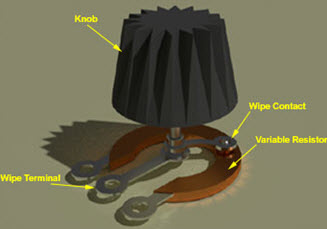
\includegraphics[width=0.35\textwidth]{laborator_01/figuri/6_potentiometru0}
		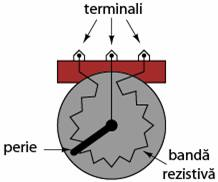
\includegraphics[width=0.3\textwidth]{laborator_01/figuri/6_potentiometru1}
	\caption{Poten'tiometrul -- mod de func'tionare} %\cite{aplicatii_potentiometru}.}
	\label{fig:potentiometru}
\end{figure}

\begin{figure}[!t]
	\centering
		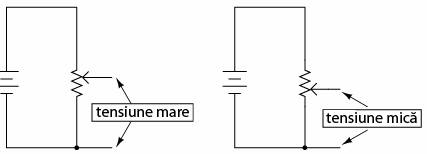
\includegraphics[width=0.65\textwidth]{laborator_01/figuri/6_potentiometru2}
	\caption{Poten'tiometrul -- tensiunea preluat'a se modific'a 'in func'tie de pozi'tia punctului de contact 'intre perie 'si banda rezistiv'a.} % \cite{aplicatii_potentiometru}.}
	\label{fig:potentiometru_tensiuni}
\end{figure}

\subsection*{Senzori rezistivi}

O mare parte din senzorii din lumea real'a sunt dispozitive rezistive \cite{aplicatii_senzori_rezistivi}. S'a lu'am exemplul unui senzor de control al luminii (fotocelul'a), care poate aprinde sau stinge becul unei veioze/lustre automat, 'in func'tie de lumina ambiental'a. Fotocelula con'tine o rezisten'ta variabil'a, propor'tional'a cu cantitatea de lumin'a captat'a.

Tensiunea fiind mult mai u'sor de m'asurat dec\^at rezisten'ta, pentru determinarea rezisten'tei fotocelulei se adaug'a un alt rezistor (cu rezisten'ta fix'a 'si cunoscut'a) 'in circuit 'in serie cu senzorul, form\^andu-se astfel un divizor de tensiune. Prin m'asurarea tensiunii de ie'sire, rezisten'ta senzorului poate fi calculat'a u'sor, folosind rela'tiile divizorului de tensiune (Fig. \ref{fig:senzor_rezistiv}).

\begin{example}
O fotocelul'a are rezisten'ta variabil'a 'intre $1~\mathrm{k\Omega}$ la lumin'a 'si aproximativ $10~\mathrm{k\Omega}$ la 'intuneric. Dac'a se monteaz'a 'in serie o rezisten't'a de valoare fixat'a la $5.6~\mathrm{k\Omega}$ 'si se m'asoar'a tensiunea de ie'sire, se poate determina valoarea rezisten'tei variabile 'si a nivelului de lumin'a asociat (tabelul \ref{tab:senzori_rezistivi}).

  \begin{center}
    \begin{tabular}{ccccc}\label{tab:senzori_rezistivi}
      Nivel lumin'a & $R_2$ (senzor) & $R_1$ (fixat) & $\alpha=\frac{R_1}{R_2}$ & $V_\mathrm{out}$ (m'asurat) \\
      \midrule
      Lumin'a & $1~\mathrm{k\Omega}$ &  $5.6~\mathrm{k\Omega}$ & $5.6$ & 0.76 V \\
      Semiobscur &  $7~\mathrm{k\Omega}$ &  $5.6~\mathrm{k\Omega}$ & $0.8$ & 2.78 V \\
      'Intuneric &  $10~\mathrm{k\Omega}$ &  $5.6~\mathrm{k\Omega}$ & $0.56$ & 3.21 V \\
    \end{tabular}
  \end{center}
\end{example}

\begin{figure}[!b]
	\centering
		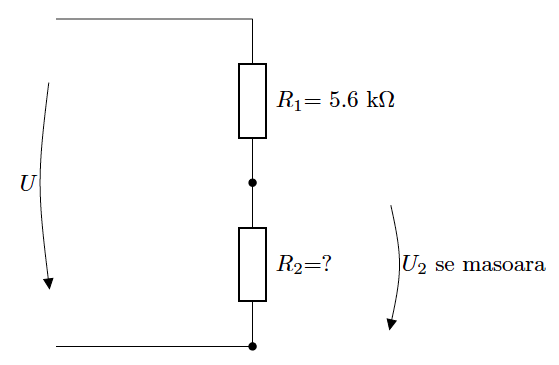
\includegraphics[width=0.45\textwidth]{laborator_01/figuri/6_senzor_rezistiv}
	\caption{Senzor rezistiv. Valoarea rezisten'tei $R_2$ a senzorului poate fi determinat'a prin crearea unui divizor de tensiune.}
	\label{fig:senzor_rezistiv}
\end{figure}

Alte exemple de acest tip sunt senzori care con'tin rezisten'te sensibile la umiditate, temperatur'a, for'te.

\subsection*{Puntea Wheatstone}

Puntea Wheatstone \cite{aplicatii_punte_wheatstone} (descris'a 'in sec'tiunea \ref{subsection:puntea_rezistiva}) a fost ini'tial dezvoltat'a de Charles Wheatstone pentru a m'asura valorile unor rezisten'te 'si ca mijloc de calibrare a instrumentelor de m'asurare (voltmetre, ampermetre).

Puntea este \textit{'in echilibru} dac'a $V_a=V_b$, ceea ce se 'int\^ampl'a dac'a rela'tia dintre rezisten'te este $R_1 R_x = R_2 R_3$. Pe acela'si principiu ca senzorii rezistivi, dac'a una dintre rezisten'te este variabil'a (de exemplu cu valoarea dependent'a de lumin'a), valoarea ei poate fi determinat'a prin echilibrarea pun'tii 'si folosirea rela'tiei 'intre rezistoare pentru o punte echilibrat'a (Fig. \ref{fig:punte_Wheatstone}).

De'si ast'azi multimetrele digitale reprezint'a cea mai simpl'a modalitate de a m'asura o rezisten't'a, puntea Wheatstone poate fi utilizat'a 'in continuare pentru a m'asura valori foarte mici ale rezisten'telor (de ordinul miliohmilor).

\begin{figure}[!t]
	\centering
		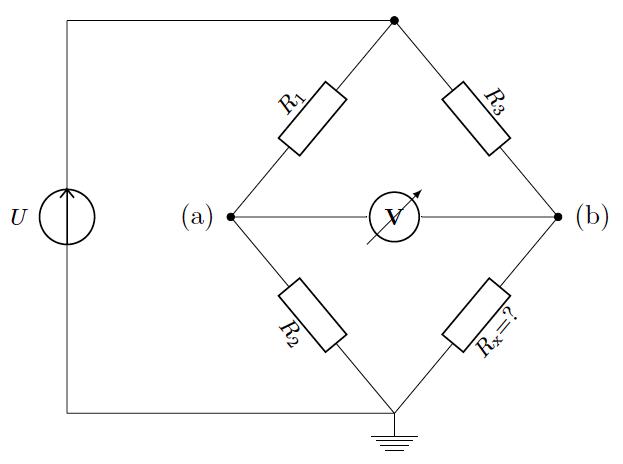
\includegraphics[width=0.45\textwidth]{laborator_01/figuri/6_punte_Wheatstone}
	\caption{Puntea Wheatstone. Valoarea rezisten'tei $R_\mathrm{x}$ se determin'a prin echilibrarea pun'tii 'si folosind rela'tia 'intre rezistoare pentru punte echilibrat'a.}
	\label{fig:punte_Wheatstone}
\end{figure}
